% !TeX spellcheck = cs_CZ
\begin{example}\label{TEMP:ex_koax_H}
  Stanovte intenzitu magnetického pole dlouhého přímého souosého kabelu podle obr.
  \ref{TEMP:fig_exam_koax}. Středním vodičem (\emph{žílou}) prochází proud $I$ a týž proud 
  opačného smyslu prochází vnějším vodičem (\emph{pláštěm}). Proudy jsou rovnoměrně rozloženy po 
  průřezech vodičů. Nakreslete graf průběhu $H = f(r)$ \cite[s.~92]{Dufek1970},
  \cite[s.~195]{Kotlan1999}.
  
  {\centering
   \begin{tabular}{cc}
     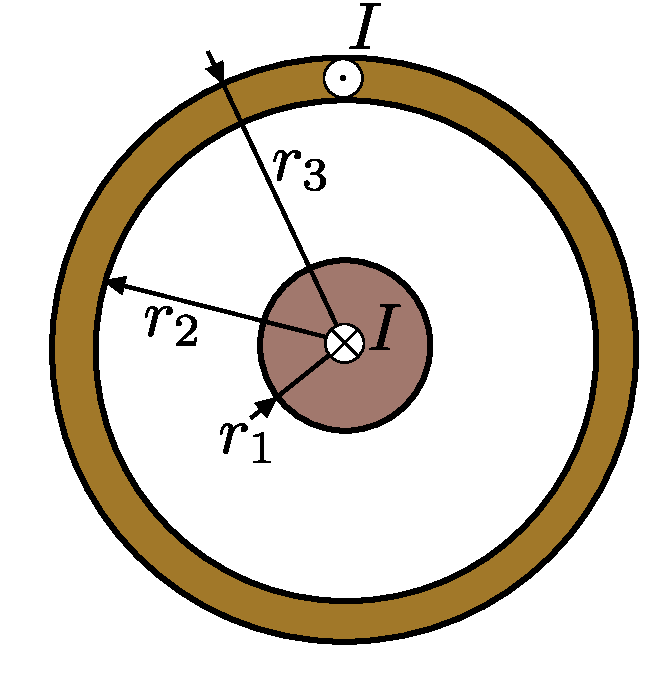
\includegraphics[width=0.4\linewidth]{vypocet_H_sousy_kabel.pdf}   &
     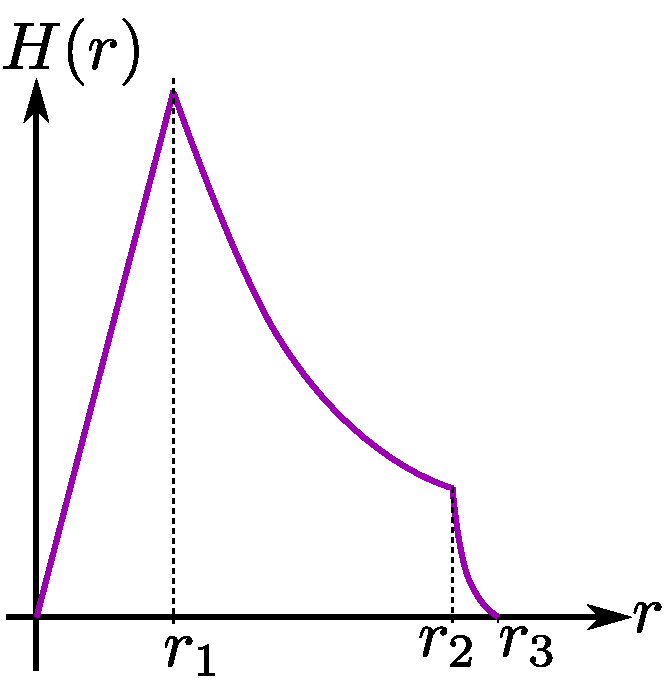
\includegraphics[width=0.4\linewidth]{koax_H_prubeh.pdf}
  \end{tabular}
  \captionsetup{type=figure}
  \captionof{figure}{K příkladu stanovení intenzity magnetického pole dlouhého souosého kabelu 
             protékaného proudem: a) náčrt; b) $H=f(r)$}
  \label{TEMP:fig_exam_koax}
  \par}
  
  \textbf{Řešení}: \newline Rovnici \ref{TEMP:eq_1MR_v_hom_p} aplikujeme na jednotlivé intervaly 
  osově souměrného stacionárního magnetického pole, přičemž se prakticky jedná o superpozici dvou
  polí. V oblasti $r<r_2$ se uplatňuje pouze pole vnitřního válcového vodiče (žíly), pro $r>r_2$ 
  přistupuje souosé pole vnějšího trubkového vodiče.
  \begin{itemize}
    \item Pro oblast $r<r_1$ je vzhledem k 
          \begin{align*}
              % \nonumber to remove numbering (before each equation)
              dI   &= \vr{J}d\vr{S} \\
              I(r) &= \int_S dI = \int_S \vr{J}d\vr{S} = \int_S J\cos\beta dS \\
                   &= \left|\begin{array}{cc}
                               \beta = 0 & H = \text{konst} \\
                             S = \pi r^2 & dS = 2\pi rdr \\
                            \end{array}
                      \right| = J\int_0^r 2\pi rdr = J\pi r^2
          \end{align*}
          hledané řešení 1. MR dáno 
          $$\oint_\mathcal{C}\vr{H}d\vr{l} = H_1 2\pi r = I(r) = J\pi r^2$$ kde celková proudová
          hustota je  $$J = \frac{I}{\pi r_1^2}$$ a tedy $$H_1 = \frac{I}{2\pi r_1^2}\cdot r$$
          
    \item Pro oblast $r_2>r>r_1$ řešíme v podstatě pole vně osamoceného válcového vodiče
          $I(r)$ a tedy $$H_2 = \frac{I}{2\pi r}$$
    \item Pro $r>r_3$ je magnetické pole vytvářeno celým proudem žíly $I$ a příslušnou částí
          proudu pláště $J\pi(r^2 - r_2^2)$, kde proudová hustota $$J =
          \frac{I}{\pi(r_3^2-r_2^2)}$$ má opačnou orientaci oproti proudové hustotě žíly. Pak 
          \begin{align*}
            I(r)                           &= I - I\frac{r^2-r_2^2}{r_3^2-r_2^2} \\
            \oint_\mathcal{C}\vr{H}d\vr{l} &= H_32\pi r = I(r)                   \\          
            H_3                            &= \frac{I}{2\pi r}\left(1 - 
            \frac{r^2 - r_2^2}{r_3^2 - r_2^2}\right) 
          \end{align*}
          Stejný výsledek dostaneme superpozicí opačně orientovaných polí $$H_3 = H'_3 - H''_3 =
          \frac{I}{2\pi r} - \frac{I}{2\pi r}\left(\frac{r^2 - r_2^2}{r_3^2 - r_2^2}\right)$$. 
  \end{itemize}
  Průběh $H(r)$ je na obr. \ref{TEMP:fig_exam_koax}.
\end{example}
